\documentclass{article}

%-----------------------------------------------PACKAGES-------------------------------------------------------------%
\usepackage{graphicx} %images
\DeclareGraphicsExtensions{.pdf,.png,.jpg} % configures latex to look for the following image extensions
\usepackage{setspace} % allows for configuring the linespacing in the document
\usepackage{caption}
\usepackage{natbib}
\usepackage[a4paper, total={6in, 8in}]{geometry}
\usepackage[explicit]{titlesec}
\usepackage[toc,page]{appendix}
\usepackage{hyperref}
\usepackage[dvipsnames]{xcolor}
\usepackage{cleveref}
\setcounter{tocdepth}{2}
\usepackage[nottoc]{tocbibind}
\usepackage[parfill]{parskip}

\usepackage{listings} % to use code snippets 
\usepackage{color}

\usepackage{glossaries} % for glossary
\usepackage[final]{pdfpages}
\makeglossaries 
\newglossaryentry{API}
{
    name={API},
    text={API},
    description={Application programming interface. A set of endpoints which lead to functions and application logic. Allows developers to expose application functionality without directly exposing the code within the application}
}
\newglossaryentry{CRUD}
{
    name={CRUD},
    text={CRUD},
    description={Create, Read, Update, Delete. CRUD defines the four cornerstones of API functionality. An API should provide these functions to any user using the API}
}
\newglossaryentry{container}
{
    name={Container},
    text={container},
    description={An isolated piece of software bundled with everything it needs to run on the host}
}
\newglossaryentry{docker}
{
		name={Docker},
    text={Docker},
		description={A piece of software which enables orchestration and management of containers on a host}
}
\newglossaryentry{docker image}
{
		name={Docker Image},
		description={A template from which many containers can be started. Can be pushed an pulled to/from a remote Docker registry}
}
\newglossaryentry{docker daemon}
{
		name={Docker Daemon},
		description={The server-side component of the Docker Engine}
}
\newglossaryentry{lifecycle management}
{
		name={Lifecycle Management},
    text={lifecycle management},
		description={The management of a container over its complete lifecycle, from its beginnings as an image to starting, stopping and restarting the container and managing the interactions it has with other containers on the system}
}
\newglossaryentry{continuous integration}
{
		name={Continuos Integration},
		description={The act of continuously merging newly created software with the current working version, validated by automatic build and testing tools allowing for early detection of faults}
}
\newglossaryentry{continuos deployment}
{
		name={Continuos Deployment},
		description={The act of continuously deploying software which has passed acceptance tests to a live system}
}
\newglossaryentry{command line}
{
    name={Command Line},
    text={command line},
    description={The program through which the operating system can be interacted with. The user enters a command they wish to execute on a text line}
}
\newglossaryentry{open source}
{
    name={Open Source},
    text={open source},
    description={Software which encourages input and feedback from other developers and allows for any and all modifications to the current software package with the intent to release it under a new package}
}
\newglossaryentry{technical debt}
{
    name={Technical Debt},
    text={technical debt},
    description={The extra development work which arises as a result of implementing an easier but less robust solution}
}
\newglossaryentry{sonarqube}
{
    name={SonarQube},
    text={SonarQube},
    description={A tool to scan source code. It can inform developers of coding best-practices and highlight ``code smells'', which are essentially when best practices are not adhered to. Also highlights technical debt. Code is deemed either `passing' or `failing', meaning the code has been deemed either sufficient or insufficient in the following categories: Code Test Coverage, Bugs, Vulnerabilities and Technical Debt Ratio}
}
\newglossaryentry{travis}
{
    name={Travis},
    text={Travis},
    description={A website which allows for automatic builds of code and feedback of results. Can be used to automatically deploy code dependent on test results also}
}
\newglossaryentry{git}
{
    name={Git},
    description={A version control system which allows source code to be tightly controlled and stored in a central repository}
}
\newglossaryentry{github}
{
    name={Github},
    text={Github},
    description={An online platform to store git repositories. Allows for multi-developer collaboration on projects}
}
\newglossaryentry{Docker Compose}
{
    name={Docker Compose},
    description={A tool developed by Docker to allow developers to easily orchestrate multi-container systems without requiring them to manually manage containers}
}
 

\definecolor{lightgray}{rgb}{.9,.9,.9}
\definecolor{darkgray}{rgb}{.4,.4,.4}
\definecolor{purple}{rgb}{0.65, 0.12, 0.82}

\lstdefinelanguage{JavaScript}{
  keywords={typeof, new, true, false, catch, function, return, null, catch, switch, var, if, const, let, in, while, do, else, case, break, require},
  keywordstyle=\color{blue}\bfseries,
  ndkeywords={class, export, exports, boolean, throw, implements, import, this},
  ndkeywordstyle=\color{darkgray}\bfseries,
  identifierstyle=\color{black},
  sensitive=false,
  comment=[l]{//},
  morecomment=[s]{/*}{*/},
  commentstyle=\color{purple}\ttfamily,
  stringstyle=\color{red}\ttfamily,
  morestring=[b]',
  morestring=[b]"
}

\lstset{
   language=JavaScript,
   backgroundcolor=\color{lightgray},
   extendedchars=true,
   basicstyle=\footnotesize\ttfamily,
   showstringspaces=false,
   showspaces=false,
   numbers=left,
   numberstyle=\footnotesize,
   numbersep=9pt,
   tabsize=2,
   breaklines=true,
   showtabs=false,
   captionpos=b
}
\usepackage{hyperref}
\newcommand\myshade{85}
\colorlet{mylinkcolor}{NavyBlue}
\colorlet{mycitecolor}{YellowOrange}
\colorlet{myurlcolor}{Aquamarine}

\hypersetup{
  linkcolor  = mylinkcolor!\myshade!black,
  linktocpage=true,
  citecolor  = mycitecolor!\myshade!black,
  urlcolor   = myurlcolor!\myshade!black,
  colorlinks = true,
}

\bibliographystyle{agsm}
\setcitestyle{authoryear,open={(},close={)}}

\begin{document}
\onehalfspacing
\hypersetup{pageanchor=false}
% !TEX root = ../final_report.tex
\begin{titlepage}
	\centering
	\mbox{}\\
	\mbox{}\\
	\mbox{}\\
	{\huge\bfseries Lifecycle Management for Docker UI \par}
	{\Large\bfseries \textit{Gantry}\par}
	\vspace{1cm}
	{\scshape\large Final Report (Semester 2)\par}
	\vspace{3cm}
	{\Large Stephen Coady\par}
	{\Large 20064122\par}
	\vspace{3cm}\par
	\vfill
	{\Large Dr.~Brenda \textsc{Mullally}}
	\vspace{1cm}\par
	{\Large BSc (Hons) in Applied Computing\par}

  % {\large \today\par}

	\vfill
	
	\clearpage
	\thispagestyle{empty}
	\centering
	\mbox{}\\
	\mbox{}\\
	\begin{figure}[!ht]
	\centering
	\includegraphics*[width=0.7\textwidth]{images/gantry-single-darktext}
	\label{fig:gantry-single-darktext}
	\end{figure}
	
	{\huge\bfseries Gantry: Lifecycle Management For Docker UI \par}
	\vspace{1cm}
	{\Large \textit{Stephen Coady}\par}
	\vspace{3cm}\par
	\vfill
	\vspace{1cm}\par

	% {\large \today\par}

	\vfill
% Bottom of the page
\end{titlepage}

\hypersetup{pageanchor=true}
\clearpage
\begin{center}
\begin{minipage}{\textwidth}
  
  {\scshape\large \textbf{Plagiarism Declaration}\par}
  \vspace{1cm}
  Unless otherwise stated all the work contained in this report is my own.  I also state that I have not submitted this work for any other course of study leading to an academic award.
\end{minipage}
\end{center}
\vfill % equivalent to \vspace{\fill}
\clearpage

\tableofcontents

\newpage
\printglossaries

\newpage
% !TEX root = ../report_v2.tex
\section{Introduction}
\label{sec:intro}
This report will aim to guide the reader through the planning and development of the Lifecycle Management for Docker \gls{UI} application. After reading this report the reader should have a clear idea of why the application was built, what was used to build it and how the process was carried out.

This application will be built using open source principles and best practices, enabling it to be maintained and improved by any developer who wishes to contribute. For this reason many of the decisions made and processes employed were done so with an open source final product in mind.

\subsection{Problem Statement}
Currently the \gls{Docker} application does not ship with any bundled \gls{UI}. When installed, it is comprised of a client and a server side component \citep{Docker2017}. The server side exposes itself through an \gls{API} and is ultimately responsible for controlling all aspects of Docker on the host such as containers, images, networks and volumes etc. The API exposed by the server-side application of the Docker Engine is consumed by the Docker \gls{CLI} which is the client side application. A graphical representation of the complete Docker engine can be seen in Figure \ref{fig:docker_engine}.

\begin{figure}[!ht]
\centering
\includegraphics*[width=0.7\textwidth]{images/docker_engine}
\caption{\em Docker Engine Components. Credit: \citep{Docker2017}}
\label{fig:docker_engine}
\end{figure}

This model is extremely versatile as it allows the developer to control any \gls{Docker daemon} (the server-side component of a Docker installation) once they have access to the command line of the host Docker is running on. In fact, if the API exposed by the Docker daemon is exposed remotely then the developer does not need access to the host's command line, instead they can directly access the API remotely.

While the \gls{CLI} gives developers full control over the server-side component of a \gls{Docker host} it also has its drawbacks.

\begin{itemize}
	\item Learning curve - the person using the command line must be familiar with typical commands used to achieve certain tasks. This precludes anybody without these skills from using Docker.
	\item Vast set of Docker commands - there are a vast number of commands available to use from the Docker CLI. This is also a learning curve as even a developer who is familiar with a CLI must first learn the Docker commands to be able to use the client-side application. 
	\item User friendliness - The command line does not produce content that is easily readable and can often format the data it is trying to present in an odd fashion depending on things like screen size etc.
\end{itemize}

\subsection{Aims and Objectives}
\label{sub:aims}
The aim of this project is to address all of these problems while also trying to increase the functionality available to anybody who wishes to use Docker.

At a high level the primary objectives of this project are:

\begin{itemize}
	\item Fully functional server-side application
	\item Expose this application through a \gls{REST}ful API.
	\item A fully functional front-end application
	\item A \gls{Docker image} built to allow easy distribution of the application
\end{itemize}

These objectives will then provide the following functionality:

\begin{itemize}
	\item A UI which will 
	\begin{itemize}
		\item allow users to manipulate images, containers etc on the host with the same capabilities as the command line
		\item allow them to do this remotely
	\end{itemize}
	\item A runnable container which has no other dependencies so that it can be run without installing the application
	\item An independent API which can be consumed by any front end application
	\begin{itemize}
		\item This will provide flexibility if the front end framework needs to be changed further down the line
	\end{itemize}
\end{itemize}




\newpage
\appendix
\section*{Appendices}
\addcontentsline{toc}{section}{Appendices}
\renewcommand{\thesubsection}{\Alph{subsection}}

\subsection{Application Repository}
\label{appendix:code}
https://github.com/StephenCoady/lifecycle-management-for-docker

\subsection{Dockerode} 
\label{appendix:dockerode_appendix}
https://github.com/apocas/dockerode

\subsection{Travis Repository} 
\label{appendix:travis}
https://travis-ci.org/StephenCoady/lifecycle-management-for-docker

\subsection{SonarQube Repository} 
\label{appendix:sonarqube}
https://sonarqube.com/dashboard/index?id=lifecyle-management-for-docker

\subsection{Sprint Retrospectives}
\label{appendix:retros}
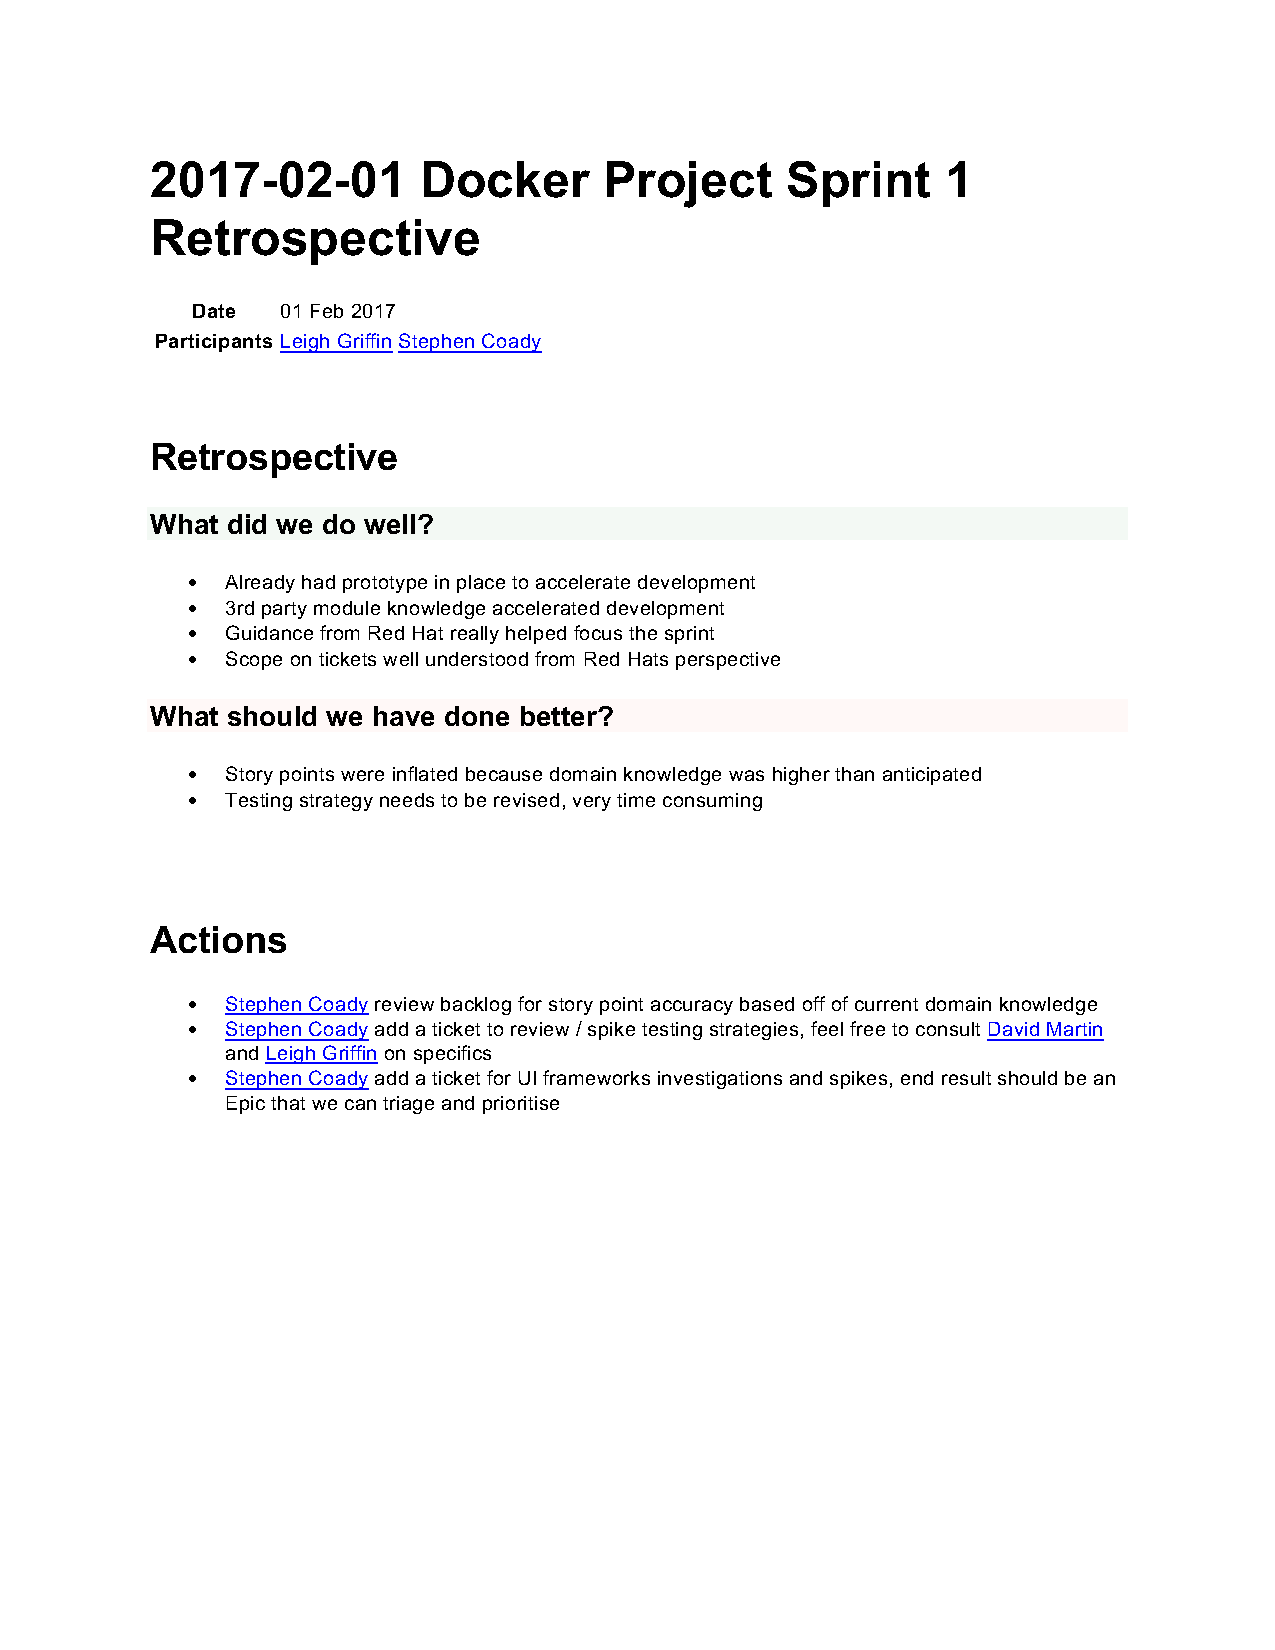
\includepdf[pages=-,pagecommand={}]{components/retrospectives/sprint_1_retrospective.pdf}


\newpage
\bibliography{bibliography}

\end{document}
